\documentclass[12pt,oneside,letterpaper]{article}
\usepackage{graphicx}

\begin{document}


\title{\bfseries Data Classifier: \\Vision and Scope}

\author {
\large{Team Mark}\\
\emph{Computer Science Department}\\
\emph{California Polytechnic State University}\\
\emph{San Luis Obispo, CA USA}\\
}

\date{October 8, 2018}
\maketitle \thispagestyle{empty}

\pagebreak
\tableofcontents

\addcontentsline{toc}{section}{Credits}

\section*{Credits}
\begin{tabular}{|l|l|p{2in}|l|}
\hline
\textbf{Name}&\textbf{Date}&\textbf{Role}&\textbf{Version}\\
\hline
Spencer Schurk&October 6, 2018&Lead Author of Business Requirements&1.0\\
\hline
Geraldo Macias&October 6, 2018&Lead Author of Scope and Limitations&1.1\\
\hline
Matt Yarmolich&October 7, 2018&Competitive Analysis&1.1\\
\hline
Brad Foster&October 7, 2018&Vision of the Solution&1.1\\
\hline
&&&\\
\hline
\end{tabular}

\addcontentsline{toc}{section}{Revision History}

\section*{Revision History}
\begin{tabular}{|l|l|p{2in}|l|}
\hline
\textbf{Name}&\textbf{Date}&\textbf{Reason for Changes}&\textbf{Version}\\
\hline
Spencer Schurk&October 6, 2018&Initial version of Section 1&1.0\\
\hline
Geraldo Macias&October 6, 2018&Initial version of Section 4&1.1\\
\hline
Matt Yarmolich&October 7, 2018&Initial version of Section 6.0&6.1\\
\hline
Brad Foster&October 7, 2018&Initial version of Vision of the Solution&1.1\\
\hline
&&&\\
\hline
\end{tabular}


\newpage

\section{Business Requirements}
\subsection{Background}
Ever-growing data sets are causing an unnecessary burden on data scientists and data analysts. As data sets are expanding, and the number of sources where these sets come from is increasing, it is becoming harder for professionals working on this data to find the information they need. Much of this work currently is done manually, and makes it very difficult for someone new coming into a data position at an existing company with a large data sets to start working productively.
\subsection{Business Opportunity}
Developing a new data classifier tool will remove many of the manual hardships involved with analyzing large, and often unorganized data sets. Instead of spending hours searching for the proper data classification a data analyst might be looking for, the new data classifier tool will allow for automated classification. This tool would allow recently hired data analysts who don't have experience with a company's complex data sets to do analysis quicker. Developing this data classifier as a web-based interface allows data scientists and data analysts to spend less time looking for the data, and more time providing useful insights and metrics to the company.
\subsection{Business Objectives and Success Criteria}
\begin{tabular}{|p{1in}|p{4.5in}|}
\hline
\textbf{BO-1}&Develop a machine-learning powered data classifier.\\
\hline
\textbf{BO-2}&Develop a web-based GUI that interfaces with the data classifier and allows edits to classification.\\
\hline
\textbf{BO-3}&Data classifications can be exported into a Data Catalog.\\
\hline
\end{tabular}
\newline
\vspace{1cm}
\newline
\begin{tabular}{|p{1in}|p{4.5in}|}
\hline
\textbf{SC-1}&Increase productivity of data scientists and data analysts.\\
\hline
\textbf{SC-2}&Classifier scales over various data sets and successfully categorizes data.\\
\hline
\textbf{SC-3}&Open-source classifier sees adoption and adaptation by outside companies.\\
\hline
\end{tabular}
\subsection{Customer or Market Needs}
\begin{tabular}{|p{1in}p{4.5in}|}
\hline
\textbf{CN-1}&Interface should be viewable from a modern web-browser.\\
\hline
\textbf{CN-2}&Machine-Learning techniques should be used to classify incoming data.\\
\hline
\textbf{CN-3}&Users should be able to edit classifications before they're stored and sent to Data Catalog.\\
\hline
\end{tabular}
\subsection{Business Risks}
No known business risks at present.

\section{User Description}
\subsection{User/Market Demographics}
Market Demographics for the Data Classification tool are wide as we are not targeting a niche group of people, but instead creating an open-source project for the anyone to use. However, the typical market demographic that we will be targeting will be between the age of 20 and 50 with a college degree in data science or a similar technical related field. In addition, the Data Classifier will be used majorly by data analysts who plan on taking raw data and classifying it by wanted aspects. 

\subsection{User Personas}
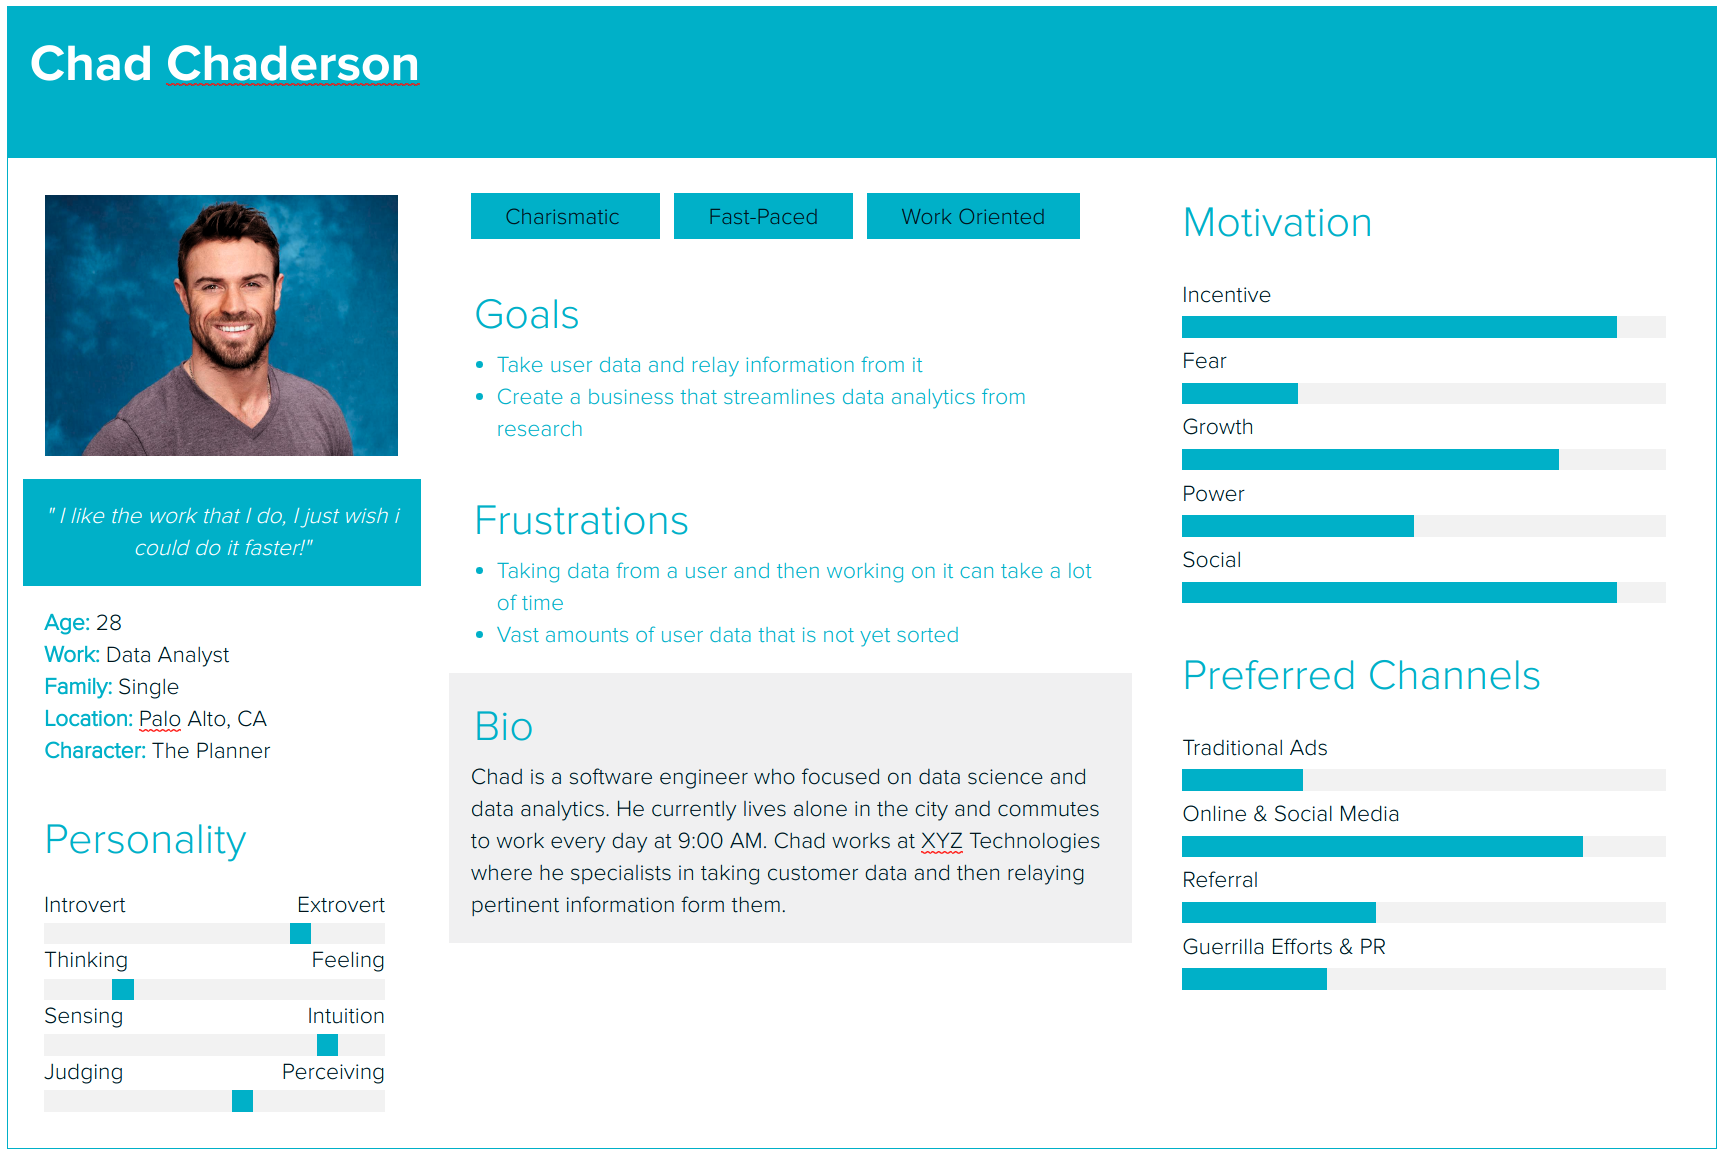
\includegraphics[scale = .35, angle = 270]{Chad.png}


\subsection{User Environment}
The User Environment is more selective and users will be using the Data Classifier while working to classify raw data for work or personal use. This service will be used by data analysts at work whenever new raw data is presented.

\subsection{Key User Needs}
Users will use this Data Classification tool to take raw data, in multiple file formats, and classify each piece so that it can be used for other tasks and in other tools afterwards. Users will need to be able to upload files and then, after processing time, be able to download a classified file from our software.


\section{Vision of the Solution}
\subsection{Vision Statement}
The solution involves a web-based interface that uses a data classifier to groom data that is sourced from various different data "silos." These silos will have data that is in various different non-standard formats.
\newline
\newline
Data analysts will be able to interact with the web interface to select parameters that will alter the presentation of the data. Through machine learning techniques, the program will make intelligent automated classifications of the data based on a respective industry. The data will also be tagged to preserve its origin.  
\subsection{Major Features}
\begin{tabular}{|p{1in}p{4.5in}|}
\hline
\textbf{FE-1}&Data analysts will provide data sets from various sources.\\
\hline
\textbf{FE-2}&The Data Classifier will use machine learning to consolidate data categories.\\
\hline
\textbf{FE-3}&The Data Classifier will output in a machine-readable standardized format.\\
\hline
\textbf{FE-4}&Data analysts will be able to use the web interface to change the presentation of the data.\\
\hline
\end{tabular}
\subsection{Assumptions and Dependencies}
\begin{tabular}{|p{1in}p{4.5in}|}
\hline
\textbf{FE-1}&Users of the Data Classifier will have an account with MarkLogic.\\
\hline
\end{tabular}



\newpage
\section{Scope and Limitations}
\subsection{Scope of Initial and Subsequent Releases}
405 initial release targets.
\begin{enumerate}
    \item Develop machine learning Python program which can detect different types of field types and classify different datasets.
    \item Create basic front end which can execute the python program on local datasets.
\end{enumerate}  
406 release 1 targets.
\begin{enumerate}
    \item The system will prompt the user to verify the contents and label of dataset columns. This edit will be applied and improve the machine learning on future datasets.
    \item The system will catalog the each dataset according to a type defined by the machine learning algorithm.
    \item A data scientist user may search for datasets which include specific fields, or search by types of datasets.
\end{enumerate}
406 release 2 targets.
\begin{enumerate}
    \item The system will allow account creations with different permission settings.
    \item The system will redact sensitive information according to account permission settings. A system administrator will have the highest privilege to information but no modification privileges. A data scientist will have some data redacted but modification privileges. An employee will have minimal data access and no modification privileges.
\end{enumerate}
\subsection{Limitations and Exclusions}
\begin{enumerate}
    \item All datasets will be of a .csv file type.
    \item Datasets must be stored within customers maintained database.
\end{enumerate}




\section{Business Context}
\subsection{Stakeholder Profiles}
\subsection{Project Priorities}
\subsubsection{Release 1}
\subsection{Operating Environment}

\section{Competitive Analysis}
\subsection{Overview}
Right now in terms of data classifiers, there are not a ton of viable competitors besides some open source plugins and Impervia, which is a product that specialized in data classification. this product is mature and interfaces with multiple databases such as Oracle, Microsoft SQL, SAP Sybase, IBM DB2 and MySQL.  \subsection{Impervia Data Classifier}
Impervia appears to be the biggest at market competitor being the first Google search result and seem to have a fair amount of existing marketable customers. Regarding features they are a post database entry classifier meaning you log into your database after logging in and analyze what is currently stored in that database. This differentiates this solution from the solution for MarkLogic as the solution for MarkLogic is meant to serve as a buffer between the input data and the database.  Regarding pricing, Impervia seems to offer the tool for free but then charges for additional use and training for the product. 


\subsection{Scikit-learn}
Another competitor for our solution for MarkLogic is Scikit-learn and TensorFlow. These are open source plugin for Python which allows you to train a MachineLearning model for datasets. In terms of marketing/marketability, since these products are open source, it is available for both commercial and private use for free. This means these product are not a direct competitor to our solution for MarkLogic, and can probably be used in our implementation pending on the desired feature set. 

\subsection{Conclusion}
In conclusion there are not a ton of commercially viable solutions for MarkLogic that we will be competing with. Most existing solutions require a team of Software Engineers to train the model and build it into a usable tool. 


\end{document}
